\documentclass[11pt]{article} % use larger type; default would be 10pt


%%% PAGE DIMENSIONS
\usepackage[top=1in, bottom=1in, left=0.5in, right=0.5in]{geometry} % to change the page dimensions
 
%%% PACKAGES
\usepackage{graphicx} % support the \includegraphics command and options
\usepackage{amsfonts}
\usepackage{amsmath}
\usepackage{tikz}
\usepackage{graphicx}
\usepackage{color}
\usepackage{bbm}
\usetikzlibrary{arrows}
 

%%% The "real" document content comes below...

\title{CS 134: Networks \\ \emph{Problem Set 10}}
\author{Xiner Zhou}
\date{\today} % Activate to display a given date or no date (if empty),
        

\begin{document}
 
\maketitle

\paragraph{1. Suboptimality of $k$-means (Understanding Machine Learning, 22.8 Q1) (20 points)}

\textcolor{red}{Solution:} 
\begin{center}
	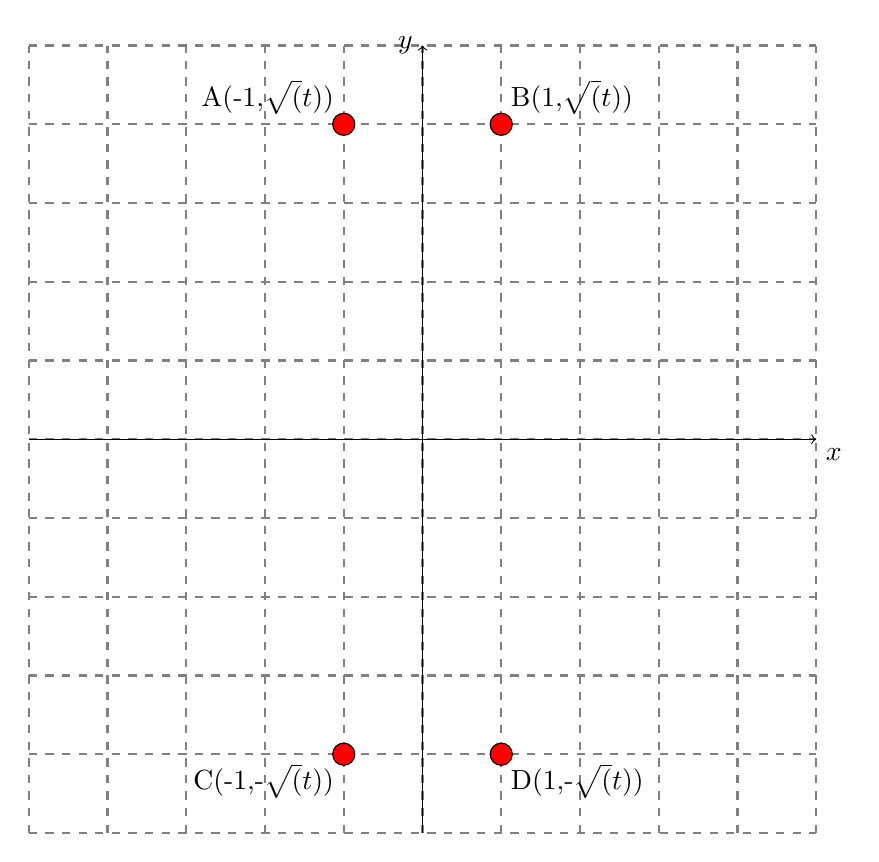
\begin{tikzpicture}
		\draw[thick, color=gray, step=1cm, dashed] (-5,-5) grid (5,5);
		\draw[->] (-5,0)--(5,0) node[below right] {$x$};
		\draw[->] (0,-5)--(0,5) node[left] {$y$};

		\coordinate (A) at (-1, 4);
		\coordinate (B) at (1, 4);
		\coordinate (C) at (-1, -4);
		\coordinate (D) at (1, -4);
		
		\draw[fill=red] (A) circle (4pt) node[above left]{A(-1,$\sqrt(t)$)};
		\draw[fill=red] (B) circle (4pt) node[above right]{B(1,$\sqrt(t)$)};
		\draw[fill=red] (C) circle (4pt) node[below left]{C(-1,-$\sqrt(t)$)};
		\draw[fill=red] (D) circle (4pt) node[ below right]{D(1,-$\sqrt(t)$)};

	\end{tikzpicture}
\end{center}

For $\forall t>1$, suppose $X =\{ A(-1, \sqrt{t}), B(1, \sqrt{t}), C(-1, -\sqrt{t}), D(1, -\sqrt{t}) \} \subseteq R^2$, let the number of clusters $k=2$. Then, the optimal partition of X that minimizes the objective function is 
$$C_1=\{A,B\} \ C_2=\{C,D\}$$
$$\mu_1=(0, \sqrt{t}) \ \mu_2=(0, -\sqrt{t})$$
the minimal objective function value is: 
$$OPT=\sum_{i=1}^{2} \sum_{x \in C_i} d(x, \mu_i)^2=1+1+1+1=4$$.

However, if choose the initial centroids at $\mu_1=(-1, 0)$,$\mu_2=(1, 0)$, then the k-means algorithm will stuck at the local maximum and returns the convergence: 
$$C_1=\{A,C\} \ C_2=\{B,D\}$$
$$\mu_1=(-1, 0) \ \mu_2=(1, 0)$$
the objective function value is: 
$$objective=\sum_{i=1}^{2} \sum_{x \in C_i} d(x, \mu_i)^2=t+t+t+t=4t=t \times OPT$$.

Since t is an arbitrary real greater than 1, we can stretch vertically for any value of t which gives an instance of the k-means problem for which the k-means algorithm might (depends on initial centroids) find a solution whose k-means objective is at least $t \times OPT$, where $OPT$ is the minimum k-means objective.
 
 
\paragraph{2. $k$-means Might Not Necessarily Converge to a Local Minimum (Understanding Machine Learning, 22.8 Q2) (20 points)}

\textcolor{red}{Solution:} 

The example made in Q1 has already shown that the k-means algorithm might converge to a point which is not a local minimum, and even worse can bve arbitrarily "bad" in terms of the minimum objective function. \\

Another example given by the hint: Soppose that $k=2$ and the sample points are $\{1,2,3,4\} \subseteq R$, suppose we initialize the k-means with the centers $\{2,4\}$; and suppose we break ties in the definition of $C_i$ by assigning $i$ to be the smallest value in $argmin_j ||x-\mu_j||$. Then the algorithm converges after 1 iteration and returns: 
$$C_1=\{1,2,3\} \ C_2=\{4\}$$
$$\mu_1=2 \ \mu_2=4$$
the objective function value is: 
$$objective=\sum_{i=1}^{2} \sum_{x \in C_i} d(x, \mu_i)^2=1+0+1+0=2 \times OPT$$.

However, the local minimum is given by: 
$$C_1=\{1,2 \} \ C_2=\{3,4\}$$
$$\mu_1=1.5 \ \mu_2=3.5$$
the objective function value is: 
$$objective=\sum_{i=1}^{2} \sum_{x \in C_i} d(x, \mu_i)^2=0.5^2+0.5^2+0.5^2+0.5^2=1 \times OPT$$.

The above two examples both show that the k-means algorithm might converge to a point which is not a local minimum.
 
\paragraph{3. Ethics, revisited (30 points)} 

\textcolor{red}{Solution:} 

One of the strategies Facebook has been implementing to address the issue of fake news and hoaxes is flagging stories as disputed. This strategy falls into the category of "soft censorship", in contrast to the "hard censorship" which is to delete what they believe as fake news. The purpose of this action to provide more context to help people decide for themselves what to trust and what to share. In order to detect news as potentially fake, they have made it easier to report a hoax by clicking the upper right corner of a post, and theyuse the reports from Facebook community to send to third-party fact checking organizations. If the fact checking organizations identify a story as fake, it will get flagged as disputed adn there will be a link to the corresponding article explaining why. Stories that been disputed may also appear lower in News Feed. 

I believe that Facebook is morally obligated to suppress the spread of fake news. According to Wiki, "Fake news" is a type of hoax or deliberate spread of misinformaiton(false information), be it via the traditional print or broadcasting news media or via Internet-based social media. To quantify as fake enws, a story has to be written and published with the intent to mislead in order to gain financially or politically". It's different from what John Stuart Mill's arguments on "On Liberty", in which Mill made strong arguments to defence the liberty of free speech as one of the securities against corrupt or tyrannical government. But what we are talking today to suppress the spread of "fake news" is totally distinct from the right of free speech. We are not arguing taking away the opportunity to express personal opinions, even deemed as contradictory or minority.  

The major argument to support my claim from the lecture, is that fake news is harmful for democracy. Democracy is supposed to work in the following way: Individuals try to figure out what is the interest of the society, and what are their own interests, then use those information to decide who should they vote for. If voters relie on misinformation, it will interfere the function of democracy. There are several reasons. First, if voters have misinformation about candicates' policies, they will be less likely to favor good policies of good candicates (good being beneficial, fair, and just) ; second, if voters favor worse candicates, the government would be less likely to implement good policies; third, the viral spread of fake news causes voters to base their policy and candidate preferences on misinformation; and finally, the viral spread of fake news makes it less likely that the government will implement good policies.   




\paragraph{4. Investigating Parameters of K-Means (30 points)}
 
\begin{enumerate}
    \item[\textbf{a.}] 
\textcolor{red}{Solution:} 
There are 2,992 nodes and 4,046 edges in the network.

    \item[\textbf{b.}]  
\textcolor{red}{Solution:} 
The average shortest pairs distance among all pairs is 11.51. 
  

    \item[\textbf{c.}]  
\textcolor{red}{Solution:} 
The distance between node 5 and the cluster $\{2,8,20\}$ under then min metric is 2; under the max metric is 4; and under the mean metric is 3.

    \item[\textbf{d.}] 
\textcolor{red}{Solution:} 
Give node 5 and clusters $\{ \{2,8,20\}, \{3,4,8,26\} \}$, the assign returns 1(the second cluster) for the min metric, 0(the first cluster) for the max metric, and 1(the second cluster) for the mean metric.


    \item[\textbf{e.}] 
\textcolor{red}{Solution:} 
Give cluster $\{2,3,4,8,20,26\}$, the node 3 is the center of the cluster.


    \item[\textbf{f.}] 
\textcolor{red}{Solution:} Please see "pset10 Code Xiner Zhou.py".

    \item[\textbf{g.}]  
\textcolor{red}{Solution:} 

As k increases, the objective function value decreases, the reason is that by allowing for more centers, each node has shorter distance to its assigned cluster centroid; and as the metric goes from min to mean, the objective funciton also decreases, the reason is that the metric "mean" assures groupings that have shorter distance between every node to the centroid overall, not just the "minimum" or "maximum" ones, therefore, make the overall cost or objective function less. 



\textbf{Run 1:}
$$\begin{array} {|c c c | c| c |c|} \hline
\text{clusters $K$} & \text{Metric} & \text {Iterations} & \text {Centers} & \text {Objective} & \text{Clusters Size}  \\ \hline
3 & min & 20 & $\{6, 1242, 353\}$ & 3,380,460 & $\{47061, 9601, 3121\}$\\  \hline 
3 & max & 20 & $\{ 6, 17, 146\}$ & 3,369,622 & $\{23808, 18126, 17849\} $\\  \hline
3 & mean & 20 & $\{58, 146, 6\}$ & 2,950,252 & $\{15407, 25582, 18794\}$ \\   \hline

5 & min & 20 & $\{458, 6, 14, 1093, 386\}$ & 3,588,200 & $\{16141, 23981, 18681, 141, 801\}$ \\  \hline
5 & max & 20 & $\{30, 805, 146, 877, 297\}$  & 3,370,356 & $\{23756, 4156, 12903, 11082, 7848\}$\\    \hline
5 & mean & 20 & $\{650, 23, 6, 80, 57\}$  & 2,664,594 & $\{15321, 14346, 7931, 13188, 8959\}$ \\    \hline

10 & min & 20 & $\{358, 6, 310, 1091, 981, $ & 3,450,920 & $\{681, 54361, 581, 101, 41,  $ \\ 
  &  &   & $ 699, 293, 1553, 317, 943\}$ &   & $ 1581, 341, 101, 941, 921\}$ \\ \hline
 

10 & max& 20 & $\{567, 20, 296, 105, 6, $ & 2,197,646 & $\{5458, 5718, 4848, 3168, 6154,  $ \\   
 &  &  & $ 57, 79, 35, 67, 373\}$ & 2,327,528 & $5875, 7808, 9168, 6097, 5356\}$ \\  \hline

10 & mean & 20 & $\{419, 57, 146, 23, 363,  $ & 2,014,012 & $\{ 6230, 5331, 9706, 6168, 7302,  $ \\ 
 &   &   & $ 124, 490, 458, 81, 33\}$ & 2,037,563 & $2311, 6805, 8153, 4877, 2767\}$ \\ \hline

20 & min & 20 &  $\{335,68,17,1832,19, $ & 2,654,612 & $\{701,3401,8221,1,9401,8481, $ \\ 
 &  &   &  $ 430,664,1060,317,58, $ &  & $ 121,15881,861,3721,1441, $ \\ 
  &  &    &  $ 386,358,155,318,1701, $ &   & $ 961,741,241,821,221, $ \\ 
  &   &   &  $ 1071,1639785,901,848\}$ &   & $ 1401,1641,461,741\}$ \\ \hline

20 & max & 20 & $\{ 1242, 510,57,326,458,$ & 1,743,943 & $\{3578,1153,6696,1853,2309, $ \\   
 &   &   & $321,566,39,350,213,$ &   & $ 1386,3015,2614,4268,1236,$ \\   
  &   &   & $ 34,33,490,365,124, $ &  & $ 5011,3308,4085,2287,2530,$ \\   
  &  &   & $1060,533,155,207,363\}$ &   & $ 4339,1642,1892,3803,2455\}$ \\    \hline

20 & mean & 20& $\{450,280,75,935,142,$ & 1,447,273& $\{2034,1663,2992,4107,1304, $ \\
 & &  & $363,34,39,215,961,$ &  & $ 3339,3683,3895,4693,2176,$ \\
 &  &  & $62,86,23,443,467,$ &   & $ 2780,2658,3334,3299,4865,$ \\
 & &  & $482,286,46,207,314\}$ &   & $ 2539,541,3373,2658,3527\}$ \\ \hline
 
\end{array}$$

   
































\textbf{Run 2:}
$$\begin{array} {|c c c | c| c |c|} \hline
\text{clusters $K$} & \text{Metric} & \text {Iterations} & \text {Centers} & \text {Objective} & \text{Clusters Size}  \\ \hline

3 & min & 20 & $\{920, 317, 3\}$ & 3,530,440 & $ \{37621, 1041, 21121\} $\\  \hline 
3 & max & 20 & $\{6, 65, 7\}$ & 3,527,003 & $\{29003, 9057, 21723\} $\\  \hline
3 & mean & 20 & $\{539, 14, 34\}$ & 3,132,819 & $\{21823, 9725, 28235\}$ \\   \hline

5 & min & 20 & $\{6, 189, 693, 365, 35\}$ &  3,656,044 & $\{41821, 4541, 661, 521, 12201\}$ \\  \hline
5 & max & 20 & $\{14, 146, 30, 19, 10\}$  & 2,852,775 & $\{17199, 21931, 5676, 11335, 3604\}$\\    \hline
5 & mean & 20 & $\{17, 61, 57, 86, 23\}$   & 2,774,238  & $\{13047, 4784, 9507, 13776, 18631\}$ \\    \hline

10 & min & 20 & $\{902, 17, 582, 650, 463, $ & 3,120,870& $\{3121, 15181, 4161, 24821, 61,$ \\ 
  &  &   & $ 443, 177, 68, 292, 720\}$ &   & $  3081, 2041, 3601, 1, 3581\}$ \\ \hline
 

10 & max& 20 & $\{31, 105, 350, 28, 297,$ &  2,144,108 & $\{2488, 5358, 4411, 10052, 10229, $ \\   
 &  &  & $ 34, 30, 23, 39, 373\}$ & 2,327,528 & $ 6979, 4366, 6947, 4598, 4223\}$ \\  \hline

10 & mean & 20 & $\{57, 296, 467, 124, 65, $ & 2,009,398 & $\{ 5468, 5132, 9059, 2531, 8768,$ \\ 
 &   &   & $ 931, 768, 419, 39, 183\}$ & 2,037,563 & $ 5318, 6057, 6552, 5396, 5369\}$ \\ \hline

20 & min & 20 &  $\{146,1403,3,117,539,$ & 2,878,866 & $\{29741,41,17541,1201,1501,$ \\ 
 &  &   &  $ 1732,142,1690,2984,319, $ &  & $41,1362,1821,61,2801,$ \\ 
  &  &    &  $454,2639,642,141,787, $ &   & $ 481,1,501,1,481,$ \\ 
  &   &   &  $1494,1487,164,312,1687\}$ &   & $ 141,61,1261,341,81\}$ \\ \hline

20 & max & 20 & $\{ 167,510,28,179,109,$ & 1,619,017& $\{3510,3271,4330,997,2899,$ \\   
 &   &   & $296,183,386,1230,33,$ &   & $3092,3874,2021,1717,4025,$ \\   
  &   &   & $ 34,451,769,39,124, $ &  & $  2863,3561,1897,4925,2361,$ \\   
  &  &   & $35,121,86,23,105\}$ &   & $2846,1729,3521,2753,3268\}$ \\    \hline

20 & mean & 20& $\{166,566,114,350,857,$ & 1,446,628 & $\{2845,3280,4301,4844,2445, $ \\
 & &  & $183,336,75,124,1431,$ &  & $3528,4311,2988,1721,2167,$ \\
 &  &  & $35,120,83,105,621,$ &   & $2333,1970,2946,2100,2708,$ \\
 & &  & $117,207,69,23,1507\}$ &   & $2076,2973,2348,4001,3575\}$ \\ \hline
 
\end{array}$$
 
   
    
 

  








\textbf{Run 3:}
$$\begin{array} {|c c c | c| c |c|} \hline
\text{clusters $K$} & \text{Metric} & \text {Iterations} & \text {Centers} & \text {Objective} & \text{Clusters Size}  \\ \hline
3 & min & 20 & NA & NA & $NA $\\  \hline 
3 & max & 20 & $\{ 23, 6, 19\}$ & 3,244,725 & $\{26706, 20086, 12991\} $\\  \hline
3 & mean & 20 & $\{23, 39, 28\}$ & 3,064,320 & $\{27980, 21405, 10398\}$ \\   \hline

5 & min & 20 & $\{40, 35, 23, 57, 355\}$ & 2590767 & $\{12309, 7949, 17281, 6924, 15282\}$ \\  \hline
5 & max & 20 & $\{146, 28, 39, 222, 23\}$  & 2,701,776 & $\{20348, 12731, 12483, 7395, 6788\}$\\    \hline
5 & mean & 20 & NA  & NA &NA \\    \hline

10 & min & 20 & $\{23, 83, 138, 1437, 58, $ & 3,236,600 & $\{11601, 9401, 26201, 141, 9341, $ \\ 
  &  &   & $ 618, 778, 283, 189, 561\}$ &   & $ 241, 261, 321, 1921, 221\}$ \\ \hline
 

10 & max& 20 & $\{146, 30, 19, 57, 221,$ & 2,327,528 & $\{10369, 7110, 6138, 6613, 6634, $ \\   
 &  &  & $ 24, 104, 67, 35, 373\}$ & 2,327,528 & $ 3622, 421, 6009, 7494, 5240\}$ \\  \hline

10 & mean & 20 & $\{57, 35, 296, 105, 336, $ & 2,037,563 & $\{ 6109, 4736, 7566, 5738, 6197, $ \\ 
 &   &   & $ 39, 363, 67, 120, 238\}$ & 2,037,563 & $ 6105, 6205, 5156, 5396, 6442\}$ \\ \hline

20 & min & 20 &  $\{6, 296,164,1664,662,  $ & 2,564,410 & $\{11561,9941,1541,701,921,  $ \\ 
 &  &   &  $ 2213,1243,168,860,1316, $ &  & $ 21,101,2901,3741,421 $ \\ 
  &  &    &  $  345,322,467,1534,826, $ &   & $ 481,2641,6041,41,1101, $ \\ 
  &   &   &  $ 105,867,368,17,629\}$ &   & $ 2181,241,541,13861,481\}$ \\ \hline

20 & max & 20 & $\{ 830,183,238,52,117,$ & 1,595,970 & $\{2074,3999,4411,725,2495, $ \\   
 &   &   & $120,133,215,124,774,$ &   & $3214,2165,3571,2614,2733,$ \\   
  &   &   & $ 296,42,57,35,490, $ &  & $ 1685,1055,5185,3925,3176,$ \\   
  &  &   & $39,187,34,33,23\}$ &   & $4099,2082,4074,3140,3038\}$ \\    \hline

20 & mean & 20& $\{455,65,46,450,80,$ & 1,401,791 & $\{1346,5466,2929,1802,2912, $ \\
 & &  & $482,166,152,69,207,$ &  & $3215,2428,2087,2520,3033,$ \\
 &  &  & $183,1507,124,105,350,$ &   & $3835,4108,2306,3396,3800,$ \\
 & &  & $171,117,150,616,443\}$ &   & $2937,2348,3329,2913,2750\}$ \\ \hline
 
\end{array}$$

 

   
\end{enumerate}
  






 











 







 
\end{document}
